
%--------------- Personalize your document here ---------------

\author{LAVAANANTHA THAYAPARENDRAN} % Enter your name
\newcommand{\studentID}{201990251} % enter your student ID
\newcommand{\supervisorone}{James Munroe} % Enter your supervisor's name
%\newcommand{\supervisortwo}{Supervisor 2}% Leave it empty or enter your second supervisor's name 
\newcommand{\department}{DEPARTMENT OF COMPUTER SCIENCE}
\newcommand{\exam}{CMSC-6950 Final Project Report}

\title{ARGOPY Python Library} %Enter the title of your report 
\date{June, 2021} % insert a specific date	

%--------------------------------------------------------------

% This document was adapted from the
% TEMPLATE FOR PHYS250 WORKSHEET created by Alastair McLean
% URL: https://www.overleaf.com/latex/templates/phys250-worksheet-template/xxftvfhmwqdt

% Jefferson Silveira
% Email: 19jdls1@queensu.ca
% Last update: 09-Jun-2021
% If you have any questions or concerns, do not hesitate to contact me.
%--------------------------------------------------------------

\documentclass[a4paper,12pt]{article}
\usepackage[left=30mm,top=30mm,right=30mm,bottom=30mm]{geometry}
\usepackage{etoolbox} %required for cover page
\usepackage{booktabs}
\usepackage[usestackEOL]{stackengine}
\usepackage[T1]{fontenc}
\usepackage[utf8]{inputenc}
\usepackage{bm}
\usepackage{graphicx}
\usepackage{subcaption}
\usepackage{amsmath}
\usepackage{amsfonts}
\usepackage{mathtools}
\usepackage{xcolor}
\usepackage{float}
\usepackage{hyperref}
\usepackage[capitalise]{cleveref}
\usepackage{enumitem,kantlipsum}
\usepackage{amssymb}
\usepackage[square,numbers,sort]{natbib}
\usepackage[ruled,vlined]{algorithm2e}
\usepackage{listings}
\usepackage{minted}
\usemintedstyle{emacs}

\renewcommand{\listingscaption}{Algorithm}
\renewcommand{\listoflistingscaption}{List of Algorithms}


\bibliographystyle{unsrtnat}

\hypersetup{
    colorlinks,
    linkcolor={black},
    citecolor={blue!50!black},
    urlcolor={blue!80!black}
}

\linespread{1}

\newtheorem{theorem}{Theorem}[section]
\graphicspath{{figures/}}	

%----------------------------------TITLE PAGE -----------------------------------
\makeatletter
\def\maketitle{
  \begin{center}\leavevmode
       \normalfont
       
\includegraphics[width=0.35\columnwidth]{MUN.png}
       \vskip 0.5cm   
       \textsc{\large \department}\\
       \vskip 1.5cm
       \rule{\linewidth}{0.2 mm} \\
       {\large \exam}\\[1 cm]
       {\huge \bfseries \@title}\\[1 cm]
	\rule{\linewidth}{0.2 mm} \\[1.5 cm]
	 
	\begin{minipage}[t]{0.45\textwidth}
		\begin{flushleft} \large
			\emph{Author:}\\
			\@author\\
			Student ID: \studentID
		\end{flushleft}
	\end{minipage}
	\begin{minipage}[t]{0.45\textwidth}
	    \begin{flushright} \large
			\ifdefempty{\supervisortwo}{\emph{Supervisor:\\}}{\emph{Supervisors:\\}}
			\supervisorone\\
			\ifdefempty{\supervisortwo}{}{\supervisortwo\\}
		\end{flushright}
	\end{minipage}
	\vfill
	{\Large \@date\par}
   \end{center}
   %\vfill
   %\null
   \cleardoublepage
  }
\makeatother


%-------------------------------- ENDTITLE PAGE ----------------------------------

\begin{document}

\pagenumbering{gobble}% Remove page numbers (and reset to1)

\maketitle

\tableofcontents
\newpage
%\listoffigures
%\newpage
%\listoftables
%\newpage
%\listofalgorithms % List of algorithms in pseudocode format
%\newpage
%\listoflistings % List of algorithms in code format
%\newpage


\pagenumbering{arabic}% Arabic page numbers (and reset to 1)

% This is how you can organize your document
\textbf{Abstract} \newline

The scope of this project is to demonstrate the skills learned in computation tools, such as Linux operation system administration, bash scripting, git, data models and python programming with different libraries. In order to explore and apply the skill sets, a domain-specific title was chosen, and its software library packages were used to solve two different tasks. The tasks includes one computation and visualization of the computation results. \newline

\noindent Throughout these activities, it was expected to present the idea of a chosen project software library and how it can be used to solve that domain-related task. In this project, it was discussed about an open-source library package called ArgoPy, which is an ocean data repository. It can be used to call ocean data set through simple API call by using the ArgoPy python library. A python scripts were written to solve those two computation tasks and to plot the computation results as a project outcome.

\newpage

\section{Introduction}

In our daily routine, we are using computation in different areas, especially in scientific research, computation plays an important role. There are many tools to facilitate the computation needs, like writing a program to perform a task, automating the job, maintaining different versions of source code,  shared platform to work on the same project, different data models for storing data collection to be able to retrieve easily and many more. In this project, we used a few of those tools to implement a program to solve two computation tasks and to visualize the outcome.\newline 

\noindent ArgoPy is a python library for Argo data analysis. Argo is a real-time global ocean observation system that provides thousands of highly accurate data of ocean measurements on a daily basis. There are many people who work on oceanography but might have good computation fluency or not at all. ArgoPy helps all levels of people to access Argo ocean data and process it as needed. It’s developed in python, which is currently one of the most trending programming language and becoming widely used by the scientific community. Argo collects data from floats that were deployed in the ocean all over the world. Data from the floats are collected by satellite in real-time, processed, merged in a single dataset and made available as open-source to anyone through an ftp server or monthly zip snapshots \cite{argopy}.\newline

\noindent For this project's scope, a python program was developed to perform two computational tasks on Argo dataset and visualize it. For the first task, the program loads the data, converts it into the dataframe, performs some data manupilation with columns, and saves it into a csv file. The visualization program loads that CSV file and plots the temperature data on latitude, longitude, and depth axis for each month. The second task was to load the temperature, pressure and salinity data and calculate the speed of sound under the ocean at different depths. The calculation results were plotted in 2D graph along with depth.\newline

\noindent For the development, Linux OS was used with python version 3.8. Anaconda is a tool for creating a virtual environment, and it also works as a package manager. VScode was used as a text editor or IDE by connecting it to the Linux machine via ssh. All the dependencies were installed inside the virtual environment, and the packages were installed with conda and pip (python package manager). A bash script was written to automate the deployment so that the dependencies doesn’t need to be installed manually. Throughout the development phase, source code was managed in GitHub. A new repository was created in GitHub and committed and pushed the updates regularly. To maintain a clean development, task one was done in one branch and task two was done in another branch, and finally, both were merged into master.\newline
\newpage

\section{Methodology}
\subsection{Task-01}

This project includes two major tasks, each with one computation and one visualization of computation results. The first task was implemented to load the dataset from Argo by using the Argopy python API and manipulate the data. As a part of the computation, the format of the dataset was changed. Initially, it was loaded as a xarray in netCDF data model and then it was changed to dataframe as it will be easier to handle the data in two dimensional. Basically, xarray holds the data in multidimensional, and it has attributes for each data that would be useful to understand the dataset. But when converting it to dataframe those attributes will be lost. It was observed that the columns didn’t have a meaningful name, and there were many unwanted columns to process. So as a part of the data pre-processing or cleaning, those unnecessary columns were deleted and changed the remaining column names to be more descriptive. Finally, the modified dataframe was saved in the local datastore in CSV format. \newline 

\noindent For the scope of the visualization of this computation and data pre-processing, the ocean temperature variable was used along with the depth and geographical coordinate space. For the plotting, data was loaded from a csv file created and saved from previous computation tasks. The given dataset doesn’t contain a field for depth, but it has pressure data in decibar units. In ocean science, a unit of decibar of pressure can be taken as a depth in meters. A 3D scatter model was plotted with longitude and latitude on the X and Y axis and the depth on Z-axis. The scatter points were coloured according to it’s positional temperature values. The ocean temperature variation can be observed based on coordinates, ocean depth, and month of the year. In above plot, a single visualization represents a data for one month. Multiple plots were created for each month from the loaded dataset and saved to visualize the temperature variation throughout the month. To produce a final output of visualization, another function was created to combine monthly temperature plots and make a single gif file showing an animated flow of each plot.

\newpage
\subsection{Task-02}

Argo dataset contains many ocean variables such as ocean temperature, salinity and pressure. One of the ocean variables that depend on those parameters is sound speed in the ocean. In general, we know the speed of sound in the air. But when it comes to the ocean, the speed of sound will change based on temperature, salinity and depth. It’s one of the interested parameters to consider in ocean science. While using sensors that works based on the sound wave (Eg: sonar), it’s important to know the speed of sound at that area of the ocean. Therefore, the second task was focused on calculating the speed of sound. \newline

\noindent There are many equations and models that exist for sound speed calculation under the ocean. For this task, the international standard algorithm, often known as the UNESCO algorithm, was used to calculate the speed of sound \cite{xkcd}. The algorithm was programmed in a sound speed calculation script as a function. It takes temperature (units celsius), salinity (units parts per thousand) and pressure (bar) as input arguments. The pressure value in the dataset is in decibar unit, so it was converted to bar before feeding the data into the sound speed calculation function. Finally, the function output was added as an additional column into the data frame and saved as a CSV file. \newline

\noindent Following the above calculation computation process, the visualization script was developed to plot the output of the sound speed calculation. It loads the CSV file created from the previous computation script and loads the data for visualization. The visualization idiom was designed to plot depth Vs sound speed with a third parameter as temperature in one plot and salinity in another plot, so two types of sound speed plots it produces. By following the same method in task one visualization, it also generated multiple plots for each month, and finally, it combines all together into one GIF animation file that shows the sound speed visualization for each month. In such a way, finally, two GIF file were created for depth Vs sound speed with temperature and salinity throughout the year. 

\newpage


\section{Results}
\subsection{Task-01 Visualization}

\begin{figure}[ht]
    \centering
    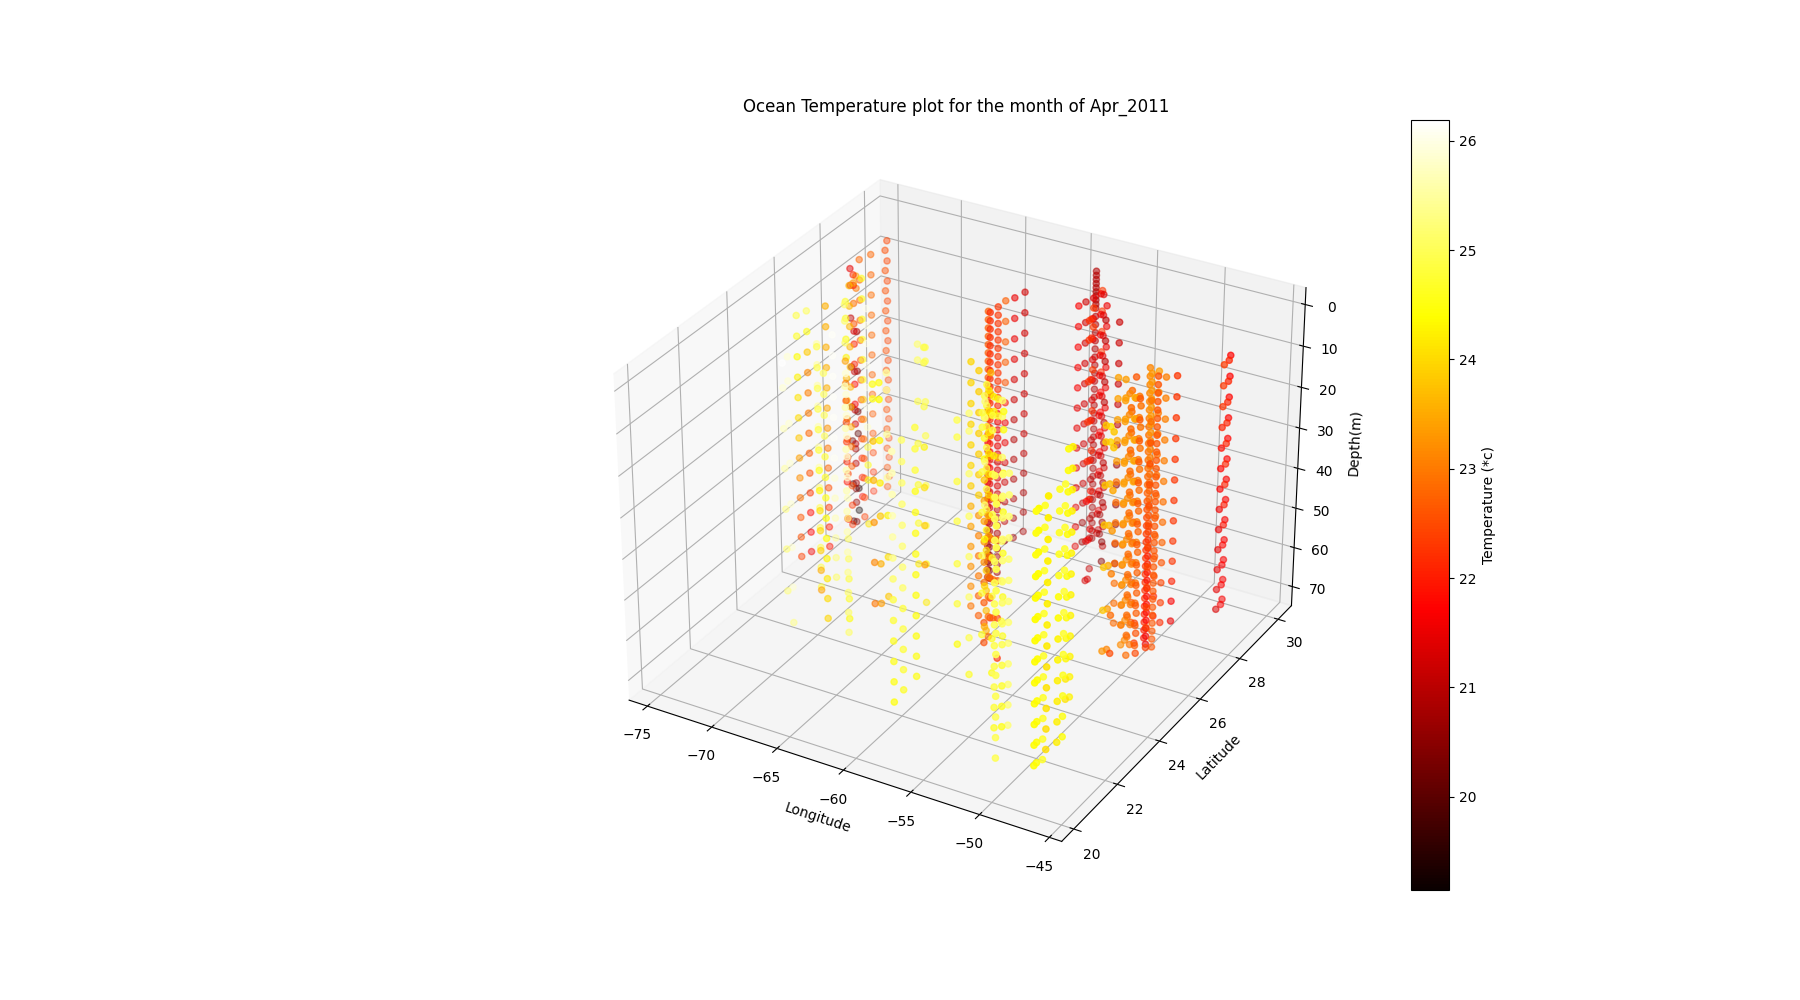
\includegraphics[width = 0.8\linewidth]{figures/oceanTemp.png}
    %\caption{You can cite the source in the caption \cite{xkcd}.}
    %\label{fig:example_1}
\end{figure}

\subsection{Task-02 Visualization}

\begin{figure}[ht] 
  \begin{subfigure}[b]{0.5\linewidth}
    \centering
    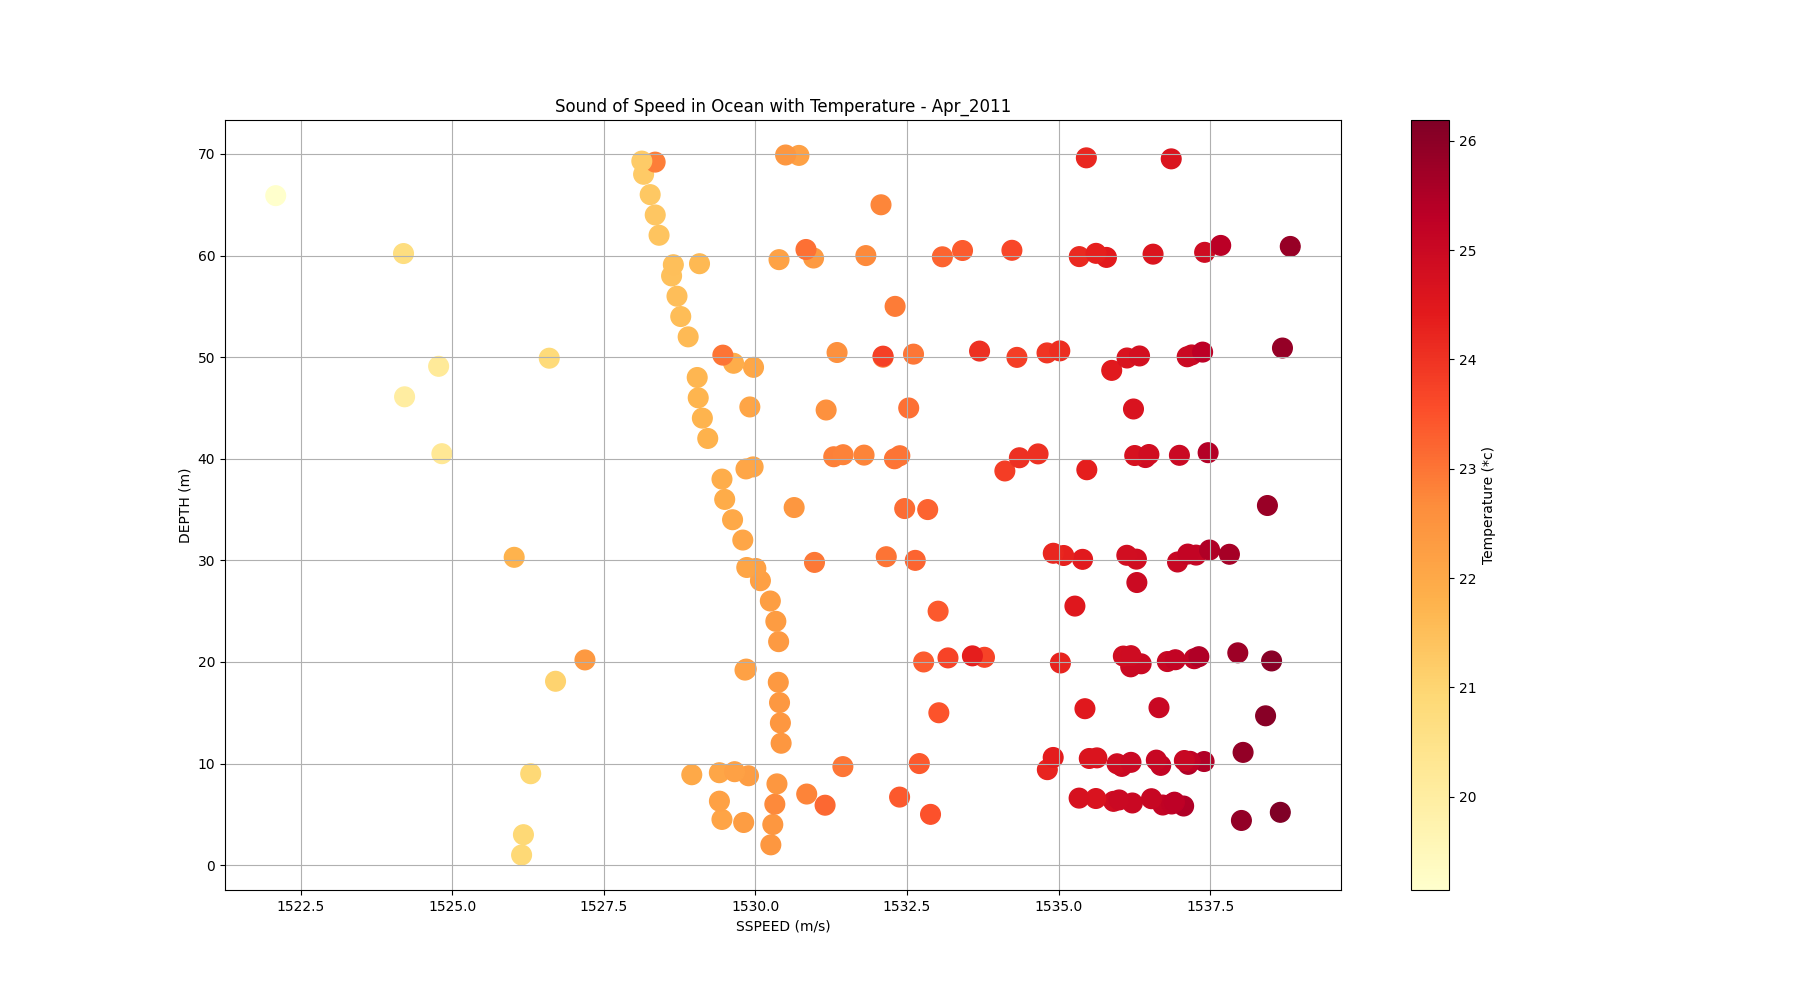
\includegraphics[width=0.9\linewidth]{figures/sspeed_temp.png}
    %\caption{Image a} 
    \label{fig:a} 
    \vspace{4ex}
  \end{subfigure}%% 
  \begin{subfigure}[b]{0.5\linewidth}
    \centering
    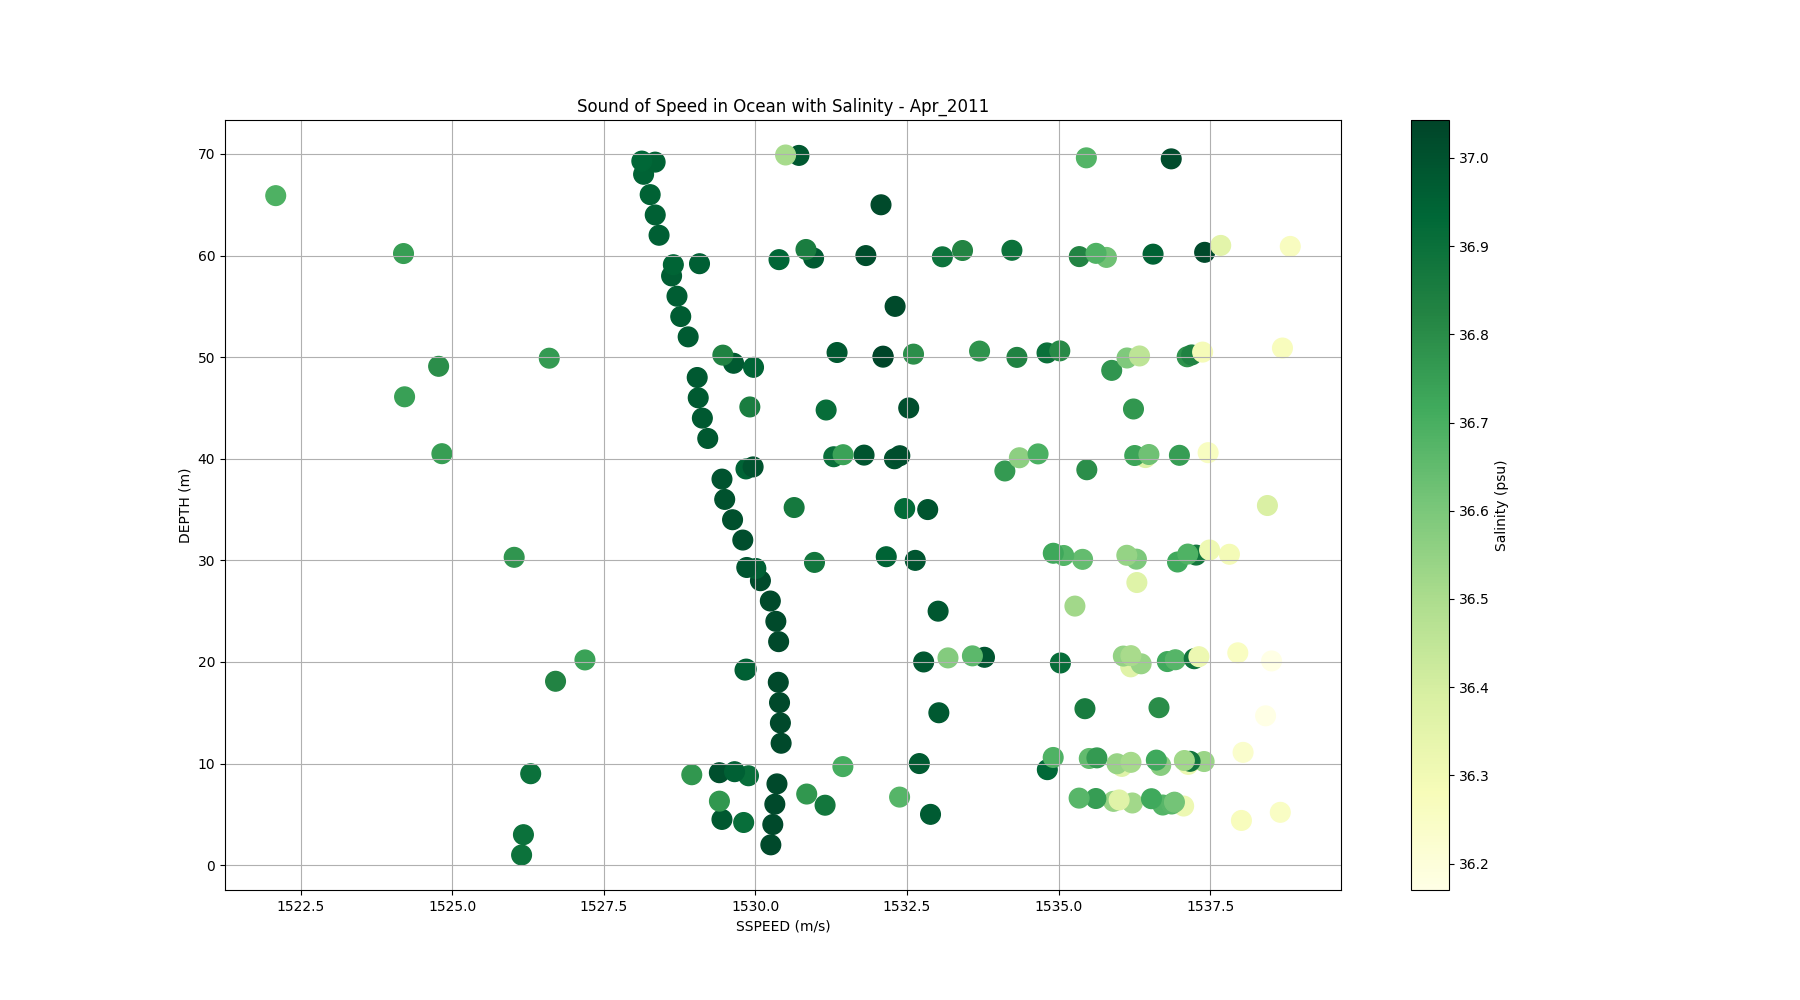
\includegraphics[width=0.9\linewidth]{figures/sspeed_sal.png} 
    %\caption{image b} 
    \label{fig:b} 
    \vspace{4ex}
  \end{subfigure} 
  %\caption{This is how you can create many images at once.}
  %\label{fig:example_many_images} 
\end{figure}

\newpage
\section{Discussion}

The field of scientific computing consists of a more complex computation process. Therefore, to facilitate it’s process for easy management and code development, it is necessary to use a supportive computation tool to make life easier. For example, bash script automation, make file, git, Github, data storage models, cloud and parallel computing are some of those tools and technologies that exist to help us work on computation models and develop solutions in more manageable way. In this project, some of those tools were used to demonstrate the learned fluency and to present the ability to work with those tools. \newline 

\noindent The project's base is the Python programming language, which is becoming trending worldwide and is the most potential and faster-growing language in the last five years[1]. It offers modern and powerful frameworks for almost all fields. Moreover, as it’s open-source, can always get community support and can see continuous growth. As argoPy also a python based software or library, it’s more convenient to work on Arogo dataset in a python program. Python works great with data and data processing. Therefore, it’s a wise decision that argo API was developed in python. \newline

\noindent ArgoPy provides the most convenient API for fetching Argo data through a simple call. By default, it uses the xarray data model. It’s an open-source Python package that helps to work easily with labelled multi-dimensional arrays. Still, it was transformed into CSV for this project's tasks as it gives a clear view of the data for calculation and visualization. Argo was developed to provide Argo data to experts and non-expert users in ocean science. So it has an option for selecting user modes as either standard or expert. Standard users can just focus on the measurements of ocean data for scientific analysis, and no need to bother about Argo's multitude of variables and parameters. The default user-mode is standard, and this entire project data was handled in standard user mode. \newline

\noindent In this project, Github was used as a version control tool and to manage the source code and for the development, VSCode IDE was used. Several packages need to be installed to set up the environment, and it was partially automated by using a bash script. Finally, to compile and execute the whole project, a makefile script was created to orchestrate the job. So all these clearly show how computation tools help in scientific computing or any other field involving computation. \newline
\newpage

\section{Conclusion}

Computation tools help in many ways as a part of the computing process. Compared to other programming languages, python is becoming more trendy and easy to use. As it already penetrated almost every technology field like web technology, data science, artificial intelligence etc., it is worth learning. Python is open-source and well maintained until up to date, so it’s more reliable and can always seek community support. Bash scripts and git tools are the most valuable components in development. With bash script, we can automate any tasks in Linux and also can use it for computation. Git is an excellent tool for source code version control and GitHub globally acts as a central portal for shared works. Can easily interact and contribute to group projects by using git. \newline

\noindent The major part of this project involves using the argopy python library. Undoubtedly, argopy fills the gap in the ocean science community by providing the most convenient approach to access a large and complex dataset which is very important in ocean science. It’s well documented and maintained by a group of developers, so anyone can easily use it for their research by simply going through the argopy documentation or user manual. The argopy developers in GitHub are so responsive and can always get support in a short period. One of the major issues faced using argopy is loading data from “Argovis” or “Errdap”, and anytime those servers can go down.
\newpage
%\input{sections/section1}
%\input{sections/examples}





%If you came here because you want your references in a new page, uncomment the following line

\clearpage % If you want the references in a separate page
\bibliography{bibliography}

%\clearpage % If you want the appendix in a separate page
%\appendix
%\input{sections/appendix}

\end{document}
